%%% The main file. It contains definitions of basic parameters and includes all other parts.

% Meta-data of your thesis (please edit)
\input metadata.tex

% Generate metadata in XMP format for use by the pdfx package
\input xmp.tex

%% Settings for single-side (simplex) printing
% Margins: left 40mm, right 25mm, top and bottom 25mm
% (but beware, LaTeX adds 1in implicitly)
\documentclass[12pt,a4paper]{report}
\setlength\textwidth{145mm}
\setlength\textheight{247mm}
\setlength\oddsidemargin{15mm}
\setlength\evensidemargin{15mm}
\setlength\topmargin{0mm}
\setlength\headsep{0mm}
\setlength\headheight{0mm}
% \openright makes the following text appear on a right-hand page
\let\openright=\clearpage

%% Settings for two-sided (duplex) printing
% \documentclass[12pt,a4paper,twoside,openright]{report}
% \setlength\textwidth{145mm}
% \setlength\textheight{247mm}
% \setlength\oddsidemargin{14.2mm}
% \setlength\evensidemargin{0mm}
% \setlength\topmargin{0mm}
% \setlength\headsep{0mm}
% \setlength\headheight{0mm}
% \let\openright=\cleardoublepage

%% If the thesis has no printed version, symmetric margins look better
% \documentclass[12pt,a4paper]{report}
% \setlength\textwidth{145mm}
% \setlength\textheight{247mm}
% \setlength\oddsidemargin{10mm}
% \setlength\evensidemargin{10mm}
% \setlength\topmargin{0mm}
% \setlength\headsep{0mm}
% \setlength\headheight{0mm}
% \let\openright=\clearpage

%% Generate PDF/A-2u
\usepackage[a-2u]{pdfx}

%% Prefer Latin Modern fonts
\usepackage{lmodern}
% If we are not using LuaTeX, we need to set up character encoding:
\usepackage{iftex}
\ifpdftex
\usepackage[utf8]{inputenc}
\usepackage[T1]{fontenc}
\usepackage{textcomp}
\fi

%% Further useful packages (included in most LaTeX distributions)
\usepackage{amsmath}        % extensions for typesetting of math
\usepackage{amsfonts}       % math fonts
\usepackage{amsthm}         % theorems, definitions, etc.
\usepackage{bm}             % boldface symbols (\bm)
\usepackage{booktabs}       % improved horizontal lines in tables
\usepackage{caption}        % custom captions of floating objects
\usepackage{dcolumn}        % improved alignment of table columns
\usepackage{floatrow}       % custom float environments
\usepackage{graphicx}       % embedding of pictures
\usepackage{indentfirst}    % indent the first paragraph of a chapter
\usepackage[nopatch=item]{microtype}   % micro-typographic refinement
\usepackage{paralist}       % improved enumerate and itemize
\usepackage[nottoc]{tocbibind} % makes sure that bibliography and the lists
			    % of figures/tables are included in the table
			    % of contents
\usepackage{xcolor}         % typesetting in color
\usepackage{longtable}
\usepackage{dirtree}

% The hyperref package for clickable links in PDF and also for storing
% metadata to PDF (including the table of contents).
% Most settings are pre-set by the pdfx package.
\hypersetup{unicode}
\hypersetup{breaklinks=true}

% Packages for computer science theses
\usepackage{algpseudocode}  % part of algorithmicx package
\usepackage{algorithm}
\usepackage{fancyvrb}       % improved verbatim environment
\usepackage{listings}       % pretty-printer of source code

% You might want to use cleveref for references
% \usepackage{cleveref}


% Set up formatting of bibliography (references to literature)
% Details can be adjusted in macros.tex.
%
% BEWARE: Different fields of research and different university departments
% have their own customs regarding bibliography. Consult the bibliography
% format with your supervisor.
%
% The basic format according to the ISO 690 standard with numbered references
\usepackage[natbib,style=iso-numeric,sorting=none]{biblatex}
% ISO 690 with alphanumeric references (abbreviations of authors' names)
%\usepackage[natbib,style=iso-alphabetic]{biblatex}
% ISO 690 with references Author (year)
%\usepackage[natbib,style=iso-authoryear]{biblatex}
%
% Some fields of research prefer a simple format with numbered references
% (sorting=none tells that bibliography should be listed in citation order)
%\usepackage[natbib,style=numeric,sorting=none]{biblatex}
% Numbered references, but [1,2,3,4,5] is compressed to [1-5]
%\usepackage[natbib,style=numeric-comp,sorting=none]{biblatex}
% A simple format with alphanumeric references:
%\usepackage[natbib,style=alphabetic]{biblatex}

% Load the file with bibliography entries
\addbibresource{bibliography.bib}

\usepackage[acronym,toc=true,automake=immediate]{glossaries-extra}
\makeglossaries
\glssetcategoryattribute{acronym}{indexonlyfirst}{false}
\setabbreviationstyle[acronym,]{long-short}


% Our definitions of macros (see description inside)
\input macros.tex

\input acronyms-and-glossary.tex

%%% Title page and various mandatory informational pages
\begin{document}
\include{title}

%%% A page with automatically generated table of contents of the thesis

\tableofcontents

%%% Each chapter is kept in a separate file
\chapter*{Introduction}
\addcontentsline{toc}{chapter}{Introduction}

\acrfull{dqm} refers to the processes, technologies, and practices used to maintain high quality in data through its lifecycle. It encompasses the acquisition, implementation, and control of data accuracy, completeness, reliability, and relevance in enterprise systems. \acrshort{dqm} ensures that data remains accurate, consistent, and accessible across all platforms and applications within an organization.

In the age of big data and advanced analytics, \acrshort{dqm} is not just a luxury—it's an imperative. It is critical for modern enterprises for many reasons, including the following:

\begin{itemize}
    \item   Informed Decision-Making
    
    High-quality data is pivotal for accuracy in decision-making. Decisions based on inaccurate or incomplete data can lead to significant financial losses and strategic missteps.

    \item   Regulatory Compliance
    
    Many industries are subject to regulations that mandate the integrity and confidentiality of data. For example, the GDPR in Europe and HIPAA in the United States impose strict guidelines on data privacy and the quality of information that is stored and processed.
        \acrshort{dqm} helps organizations comply with these regulations and avoid hefty penalties by ensuring data is managed correctly throughout its lifecycle.

    \item   Enhanced Customer Satisfaction

    Data quality directly impacts customer experience. Accurate customer data helps businesses understand their clients better, tailor their interactions more effectively, leading to improved customer satisfaction and loyalty.

    \item Operational Efficiency
    
    High-quality data reduces errors and the need for rework. For instance, accurate inventory data helps in managing stock levels efficiently, avoiding overstocking or stockouts.
    By automating data cleansing and enrichment, organizations can streamline workflows and allow employees to focus on higher-value activities rather than correcting data errors.    

    \item     Risk Mitigation

    Poor data quality is a major risk in itself—it can skew analysis, leading to misguided strategies that may harm the business.
    \acrshort{dqm} practices identify and correct discrepancies in data before they propagate through the enterprise, thereby mitigating risks associated with data handling and storage.

\end{itemize}





\chapter{Analysis}
\label{chap:analysis}

There are many benefits to having \glsxtrfull{dqm} processes in place. In fact, in today's data-driven environments, the assurance of data quality is not just a preference but a critical necessity. Organizations rely on accurate, timely, and reliable data to make informed decisions, drive strategies, and optimize operations. As such, the field of \glsxtrshort{dqm} has evolved to address these needs through sophisticated tools and methodologies. However, the effective implementation of these tools requires a deep understanding of both the tools themselves and the roles of those who interact with them.

This chapter delves into the analysis of the current landscape of \glsxtrshort{dqm}, focusing particularly on the need for programmatic access to these tools. This need stems from the growing requirement to seamlessly integrate data quality solutions into existing data pipelines, a task that typically falls within the purview of data engineers. As we explore this topic, we will discuss the challenges faced by data engineers. 

\section{Similar Solutions}

This section compares Ataccama ONE to other \glsxtrshort{dqm} tools that are designed for programmatic access, highlighting the relative strengths and limitations of each solution in terms of features, technology stack, and integration capabilities.

\subsection{Soda Core}

Soda Core \cite{sodacore} is a robust open-source tool tailored to integrate data quality checks directly into data pipelines. However, its feature set primarily focuses on:

\begin{itemize}
    \item Data Monitoring and Alerting
    
    Automatically detecting and alerting on anomalies in data as it flows through pipelines.

    \item Customizable Quality Checks

    While flexible, these are generally more basic compared to the depth provided by comprehensive \glsxtrshort{dqm} platforms.

    \item Python Integration
    
    Strong integration with Python-based data ecosystems, suitable for teams relying heavily on Python for data processing.
\end{itemize}

\subsection{Great Expectations}

Great Expectations \cite{great_expectations} offers a framework for setting up complex data validation and documentation, which is crucial for maintaining high data quality standards. Its key features include:

\begin{itemize}
\item Validation Framework

Extensive support for defining expectations about data, which can be automatically validated against data batches.

\item Data Docs

Automatically generated documentation that helps keep teams aligned on data quality standards.

\item Integration

While it offers broad integration capabilities, it requires significant setup and maintenance compared to more out-of-the-box solutions.
\end{itemize}


\subsection{Comparison with Ataccama ONE}

Ataccama ONE offers a more extensive suite of features than either Soda Core or Great Expectations. This includes advanced functionalities like Master Data Management, Data Cataloging, and enriched Metadata Management, which are not typically found in the aforementioned open-source tools. However, also the data quality features are more comprehensive, more advanced functions are included out of the box, including but not limited to: reference data checks, complex string manipulation, and set operations.

Despite its robust feature set, Ataccama’s main limitation lies in its less flexible integration with Python-based data pipelines, which is where Soda Core and Great Expectations excel due to their native Python support. This limitation is a significant drawback for data engineers who rely heavily on Python for data processing and pipeline orchestration and for this reason this thesis will focus on enhancing Ataccama's integration capabilities with Python-based data pipelines.

\section{The persona of Data engineer and their needs}

As previously noted, data engineers play a crucial role in integrating data quality tools into data pipelines. It is essential to design applications that meet the specific needs and requirements of its primary users. Therefore, any solution intended for pipeline integration must be carefully tailored to accommodate the unique needs of data engineers. This ensures that the tools not only fit seamlessly into their workflows but also enhance their efficiency and effectiveness in managing data quality across systems.

\subsection{Used technologies}

Data engineers, like any others, are working professionals. Many of them are used to working with some particular tools and technologies. It is vital to take into account the tools and technologies that data engineers are familiar with when designing a solution for them.

Although among the many data engineers, there are differences in the tools and technologies they use, there are some common tools and technologies that are used by the majority of them in today's world. It is important to realize that we should not only consider an ideal data engineer, a skilled senior, but also consider that there are many junior data engineers. Also, it is important to consider the cognitive load of new tools and technologies on data engineers. Not only should the tools and technologies be easy to learn and use, but also they should be based on familiar concepts and technologies. This way, the data engineers can focus on their work and not on learning new tools and technologies. 

The most commonly used tools and technologies by data engineers are Python, Java, Scala, and SQL. These tools and technologies are used for the development of data pipelines and the integration of data quality tools into these pipelines. For any set of data engineers, the intersection of their knowledge bases will include Python more often than anything else.

\subsection{Ease of use}

In any software, a balance between ease of use and functionality complemented by the correctness of conceptual abstraction needs to be found. As the API surface of this solution is not going to be large, not a lot of decisions will have to be made on this front. However, it is important to keep in mind that the users of the solution are data engineers, some of whom work in a consultant background. Many of them are not used to advanced language features, and abstractions have limited experience with software engineering. For this reason, it is important to keep the solution simple and easy to use, avoiding any complex constructs and patterns.

Furthermore, it should be taken into account that the library can be used outside of IDE and similar environments where code suggestion and documentation might not be available. For example, when writing integrations in the platforms discussed below such as Azure Data Factory and Data Bricks, the user will not have access to the documentation or code suggestions. For this reason, the API should be designed to be self-explanatory, and should be designed to be easy to use without the need for extensive documentation.

\subsection{Data security}

When designing data quality solutions for integration into existing data pipelines, especially those that involve interfacing with external applications or servers, security is a paramount concern. This is particularly critical when the data involved is sensitive, as is often the case in industries such as finance, healthcare, and government.

Sending data over the internet to a third-party service can be a security risk. Data security is a major concern for data engineers, and it is important to take into account the security requirements of data engineers when designing a solution for them.

When a data quality integration in a pipeline needs to access the server - an application running somewhere else - the network of the server has to be accessible. This can be a security risk as every new network endpoint provides an additional entry point for attackers. When applications within a private network start communicating with external entities, these points of interaction need to be secured, adding complexity and potential for oversight.  If the networked application has vulnerabilities, such as insufficient authentication, flawed authorization practices, or software bugs, it could be exploited by attackers to gain unauthorized access. This could lead to data breaches, data loss, or malicious data manipulation. 

Additionally, data transmitted over networks can be intercepted, viewed, or altered by unauthorized parties if not adequately protected. This risk is particularly severe if data is transmitted over unsecured or improperly secured connections, such as those not using TLS/SSL protocols. 

\subsection{Ease of configuration}

The need to access a running instance of a \glsxtrshort{dqm} application in order to run data quality tooling comes with added complexities.

First, the application needs to be configured and running. This is fine for an environment where such an application is already in use. Yet, still, it is an added complexity as part of the process is running somewhere else, so it can be more difficult to debug, monitor, and maintain.

Second, the pipeline needs to access the application over a network. This means that the application needs to be exposed to the network, which can not only be a security risk but also provide further complexities in terms of network configuration. In case of the server being accessible only on a private network, the application needs to be exposed to the network, which can, in some cases, be even out of question and make the integration impossible, or it can be an obstacle on the way to successful integration.

\section{Data pipelines and requirements for the integration of data quality tools}

Data pipelines are a crucial part of any data engineering project. Data pipelines are used to move data from one place to another and to transform data from one format to another. 

Many of the use cases for integrating data quality tools into data pipelines include the requirement to integrate with existing data pipeline or solutions. The data quality tools should support integration into commonly used data pipelines. It also follows that forcing a new data pipeline or \glsxtrfull{etl} solution is not a valid requirement. 

For example, in Ataccama, the application is intended to be connected to all the data sources and data targets using its custom connectors. To access the Ataccama engine and run any sort of evaluation of data quality rules, the data must be loaded into Ataccama ONE using a connection setup within the application,  or Ataccama can pushdown processing directly into databases or the data needs to be sent into a service set up from within the application. Either way, there is no straightforward way to process the data directly in the data stream because Ataccama current solution is oriented more toward table processing. In summary, all of these approaches present a challenge for integrating Ataccama into existing data pipelines.

\subsection{Pipelines in commonly used data platforms}

Modern data ecosystems are diverse, with organizations leveraging a variety of data storage solutions and computing environments to manage and analyze data. Here’s how Python integration plays a critical role across commonly used platforms:

\begin{itemize}

\item  Snowflake

Snowflake\cite{snowflake} supports multiple programming languages, including Java and .NET, but Python remains a popular choice due to its extensive library support and community.

Python is well-supported in Snowflake through connectors like Snowflake Connector for Python, which allows executing SQL statements and performing data manipulations directly from Python scripts.

\item AWS Glue

AWS Glue\cite{aws_glue} supports Python and Scala. Python, being one of the main languages supported by AWS Glue, benefits from seamless integration with other AWS services.

Python scripts in AWS Glue can perform \glsxtrshort{etl} tasks effectively, which can be developed and debugged directly in Python using Glue’s development endpoints.

\item Azure Data Factory

Azure Data Factory\cite{azure_data_factory} supports custom activities in various languages, but Python’s use in Azure functions for custom processing activities is notable due to its simplicity and effectiveness.

Python in ADF can be used to orchestrate complex data workflows, invoking Python-based processes as part of the data integration pipelines.

\item Databricks

Databricks\cite{databricks} offers a unified analytics platform that supports Python, Scala, SQL, and R. Python’s integration, particularly with PySpark for big data processing, makes it a primary choice for many developers.

Python is extensively used in Databricks notebooks for data exploration, visualization, and machine learning, highlighting its versatility and ease of use.

\end{itemize}

Given the need to operate within commonly used compute platforms such as the above-mentioned, it is imperative to consider the compatibility of programming languages supported by these environments. Each platform offers support for various technologies; however, Python stands out due to its universal acceptance and extensive integration capabilities across these systems. Whether it is executing complex data manipulation tasks in Snowflake, orchestrating \glsxtrshort{etl} processes in AWS Glue, running custom activities in Azure Data Factory, or performing data analysis and machine learning in Databricks, Python is consistently supported. 

Therefore, focusing on Python to implement data quality rules not only aligns with the operational capabilities of these platforms but also ensures that our solutions are versatile and adaptable across different technological ecosystems. This strategic choice maximizes the utility and reach of our \glsxtrshort{dqm} tools, making them accessible and functional within the predominant data processing frameworks employed by contemporary organizations.

\section{Enhancing Ataccama's Integration Capabilities}

While Ataccama offers a rich set of data quality management features, one critical area where enhancement is needed is in its programmatic accessibility. This thesis sets out to address this limitation by focusing on the development of methodologies that will enable better integration into automated data environments, particularly through the reimagination of Ataccama’s data quality expression language.

The core of this enhancement strategy involves reimplementing Ataccama's expression language in a way that maintains full compatibility with the original system. The intention is not to build entirely new features but to translate the existing capabilities into forms that are more accessible for programmatic use. This effort requires careful consideration to ensure that all functionalities remain consistent with Ataccama’s established methods, thus preserving the integrity and reliability of the platform while extending its usability.

This focus on reimplementing the expression language aims to facilitate the direct application of Ataccama's powerful data quality rules within more diverse programming environments. By doing so, the project seeks to bridge the gap between Ataccama’s robust data management tools and the practical, operational needs of modern data pipelines, making it more adaptable for data engineers who need to incorporate sophisticated data quality checks directly into their workflows. The outcome will be a more flexible tool that fits seamlessly into existing data infrastructures, enhancing Ataccama’s integration capabilities while upholding the essence of its trusted features.


\section{Ataccama Expression Language}

To facilitate the integration of Ataccama's data quality rules, a thorough understanding of the Ataccama Expression Language is essential. Below is an overview of the language components, types, and operational logic.

\subsection{Anatomy of an expression}

The structure of an expression in Ataccama's language consists of:

\begin{itemize}

\item Statements

    \begin{itemize}
        \item Variable Assignments
        
        Variables are assigned values which can include literals, operations, or function calls.
        \item Function Definitions
        
        Optional definitions that encapsulate logic or operations reusable within the expression.
    \end{itemize}
\item Resulting Expression

This is the final part of the expression where the previously defined variables and functions are utilized to compute a result. The outcome of the resulting expression is the output of the entire expression.
\end{itemize}

\subsection{Examples of an expression}

The two following examples illustrate the structure of an expression in Ataccama's language.

\subsubsection{Simple example: Arithmetic Expression}

\begin{verbatim}
a := 10;  
b := a * 2; 
b + 5
\end{verbatim}

In this example, variables a and b are used in statements to set up values that are manipulated in the resulting expression, b + 5, which computes the final output.

\subsubsection{Complex example: Digit sum}

\begin{verbatim}
value := replace(trim(input), '-', '');
function digitSum(integer digit) { 
    set.sumExp(
        trim(substituteAll("(.)", "$1 ", toString(digit))), 
        " ", 
        (x) {toInteger(x)}
    )
}
digitSum(value) % 13 == 0
\end{verbatim}

This example demonstrates a more complex expression that includes a function definition, digitSum, which is then called in the resulting expression, digitSum(value). The expression is a simplified excerpt from a data quality rule that checks ISIN numbers for validity.

\subsection{Components of Ataccama Expression Language}

Ataccama Expression Language, also called ONE Expressions, organizes data operations and logic into a series of expressions and operands defined by a rigorous structure:

\subsubsection{Operands}

Operands in Ataccama Expressions are categorized into four main types:

\begin{itemize}
    \item  Literals
    
    These include numeric, string, or logical constants (e.g., TRUE, FALSE) and the null literal. All keywords are case-insensitive.

    \item Columns
    
    Identified by their names, which require square brackets if they include spaces. In multiple input scenarios, columns are specified using dot notation (input\_name.column\_name). If only one input is used, dot notation can be omitted.

    \item Set
    
    Used exclusively with the IN operation, representing a constant expression. Sets can only appear on the right side of the IN operation.

    \item Complex Expressions
    
    These may involve various combinations of the above operand types and function calls.
\end{itemize}

\subsubsection{Data Types and Conversions}

Operands can be of specific column types such as INTEGER, FLOAT, LONG, STRING, DATETIME, DAY, and BOOLEAN. Ataccama handles type conversions automatically, widening data types as necessary ( e.g., INTEGER - LONG - FLOAT ) to accommodate operations.

\subsubsection{Handling Null Values}

The handling of null values aligns with SQL rules, with a notable exception for the STRING data type. In Ataccama, a null string is considered equal to an empty string, impacting how comparisons and operations are performed.

\subsubsection{Variables}

Expressions in Ataccama can include sequences of assignment expressions followed by a resulting expression, separated by semicolons. The first occurrence of a variable defines its type, with subsequent references needing to conform to this type.

\subsubsection{Operations and Functions}

Ataccama ONE supports a variety of operations and functions:

\begin{itemize}
    \item arithmetic functions
    \item logical functions
    \item comparison functions
    \item set functions
    \item date functions
    \item string functions
    \item bitwise functions
    \item MinMax functions
    \item aggregating functions
    \item conditional functions
    \item conversion functions
    \item formatting functions
    \item word set operation functions
\end{itemize}

The full list of functions and their descriptions can be found in the Ataccama ONE Expressions documentation \cite{one_expressions}.

\section{Summary}

Let us summarize the goals of the project:

\subsection{Use of Python}

The solution should utilize Python for the implementation of the data quality expression language. This choice is driven by two key reasons. Firstly, Python is widely recognized and utilized among data engineers, which ensures that the tools developed are easily adoptable and integrate seamlessly into existing workflows. Secondly, Python's compatibility with various data pipeline platforms makes it an ideal candidate for ensuring that our solution can be integrated across diverse data environments efficiently, facilitating broader accessibility and practical utility.

\subsection{Simple API}

In the analysis section, we identified data engineers as the primary users of the solution. The project's main objective is to develop an API that is straightforward and intuitive for data engineers. The API should be simple and user-friendly, avoiding overly complex abstractions or advanced design patterns. For instance, object creation should be straightforward, utilizing basic constructors or simple imported functions to minimize complexity and ensure ease of use.

\subsection{Local execution}

The solution should be designed to run locally, allowing data engineers to execute data quality rules directly within their Python environments. This is relevant with respect to the need for ease of use and security. By enabling local execution, data engineers can test and validate data quality rules without the need to access external servers or applications. This approach also simplifies the development process by removing dependencies on external services, ensuring that the solution is self-contained and easily deployable in various environments.

\subsection{Compatibility with the Ataccama Expression Language}

In order to maintain compatibility with the existing Ataccama ecosystem, the Python implementation should be able to execute the same data quality rules as the original Ataccama Expression Language. This includes supporting the same set of functions, operators, and expressions to ensure that data quality rules defined in Ataccama ONE can be seamlessly executed within Python environments. The Python implementation should mirror the behavior of the original Ataccama Expression Language as closely as possible to ensure consistency and compatibility across platforms.

\subsection{Reasonable performance}

To be considered a viable alternative to the original Ataccama implementation and to similar solutions on the market, the Python implementation should be able to handle data quality rules within Python environments efficiently and effectively. The performance of the Python implementation should be within acceptable limits, where a slowdown by a factor of up to 10 times compared to alternatives might be considered tolerable for deployment, but a 1000 times slowdown would indicate serious efficiency issues that could render the solution impractical. By establishing these performance benchmarks, we can validate that the Python implementation meets minimum requirements for real-world applications, ensuring it is a viable alternative for data engineers who require programmatic access to Ataccama's data quality tools. This will be further discussed in the evaluation section.

\chapter{Design}

In the design section, we will detail the process of translating Ataccama's expression language into Python, focusing on local execution and user-friendliness. The aim is to allow data engineers to seamlessly integrate Ataccama's data quality rules into their Python workflows. This section outlines the architecture, methodologies, and tools necessary to adapt Ataccama expressions for effective use in Python environments, ensuring the solution is both practical and easy to use.

\section{Context of data transformations}

Data processing pipelines typically adhere to a structured pattern known as extract-transform-load (ETL)\cite{etl}\ref{fig:etl_process}, crucial in data management. These pipelines start by extracting data from various sources, which is then transformed through cleaning, enrichment, and aggregation processes before being loaded into a final storage destination.

This thesis specifically concentrates on this transformation step, where data quality rules can be effectively implemented and integrated.

\begin{figure}[ht]
    \centering
    \begin{tikzpicture}
        % Draw boxes
        \node[draw, rectangle, align=center, minimum height=3cm, minimum width=4cm, fill=blue!20] (extract) at (0,0) {Extract \\ \scriptsize Fetch data from multiple sources};
        \node[draw, rectangle, align=center, minimum height=3cm, minimum width=4cm, fill=green!20] (transform) at (5,0) {Transform \\ \scriptsize Clean data, Enrich data, \\ \scriptsize Aggregate data, \\ \scriptsize Apply data quality rules};
        \node[draw, rectangle, align=center, minimum height=3cm, minimum width=4cm, fill=red!20] (load) at (10,0) {Load \\ \scriptsize Store in destination};
    
        % Draw arrows
        \draw[->, thick] (extract.east) -- (transform.west);
        \draw[->, thick] (transform.east) -- (load.west);
    \end{tikzpicture}
    \caption{Diagram illustrating the ETL (Extract-Transform-Load) process.}
    \label{fig:etl_process}
    \end{figure}

\section{Interface design}

The design of the API is straightforward due to the simplicity of the public functionality it offers. Below is a diagram that outlines the public interface of the transpiler:

\begin{figure}[htbp]
    \centering
    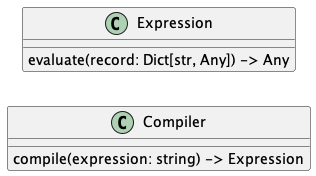
\includegraphics[scale=0.7]{diagrams/api_design-class.png}
    \caption{API overview}
    \label{fig:api}
\end{figure}

The interface is uncomplicated, designed primarily to compile and execute expressions efficiently. This simplicity ensures that all essential actions—compiling an expression and executing it—are both intuitive and accessible for users.

The API consists of two primary classes: \texttt{Compiler} and \texttt{Expression}. The \texttt{Compiler} class is responsible for compiling the expression into Python code, while the \texttt{Expression} class encapsulates the compiled code and provides a method to execute it with a given record. The record is supplied as a dictionary, where the keys correspond to the field names and the values to the field values.

\section{Architecture}

The initial step in developing the solution involves establishing its architecture, which is critical for defining how the program will function. 

The architecture of the Python implementation of the Ataccama Expression Language is designed to facilitate the translation of Ataccama's expression language into Python code to enable for local execution, one of the goals of outlined in analysis. This translation process involves parsing the input expression, generating executable code, and evaluating the expression against a dataset. The architecture is structured to accommodate these steps seamlessly, ensuring the efficient execution of data quality rules within a Python environment.

For the first step, the input expression will be converted into an abstract syntax tree (AST). Given the complexity of the expression language used by Ataccama, employing a parser generator is deemed the most effective approach. The parser generator will utilize the predefined grammar of the language to generate a parser capable of translating input expressions into an AST. This facilitates the incorporation of custom logic in the subsequent steps, particularly during the semantic analysis phase.

During semantic analysis, the AST will be traversed to construct executable code. This transformation is essential for preparing the expression for evaluation in a Python environment, from which the results can be dynamically generated and returned.

The final component of the architecture involves executing the generated code on the provided records. This step ensures that each record is evaluated according to the defined expressions, and the outcomes are systematically returned to the user.

\subsection{Parser generator}

For the parser generator, a specific approach is indicated. The Ataccama Expression Language implementation uses a parser generator called ANTLR. ANTLR (ANother Tool for Language Recognition) is a powerful parser generator\cite{antlr}. It's widely used to build languages, tools, and frameworks. From a grammar, ANTLR generates a parser that can build and walk parse trees\cite{antlr4docs}. As the grammar of the Ataccama Expression Language is already defined, it is simple and robust to use, adapt and reuse the grammar by also using ANTLR to generate the parser. 

\subsection{Code generation}

Having decided on the parser generator, the next step is to decide how to generate the code for the expression. There are two obvious approaches at hand: Represent the expression in an object tree with execution being a recursive descent through the tree. The second approach is to generate Python code directly. This can be done using Python standard module \texttt{ast}, which can be used build an abstract syntax tree of the expression, and then compile it into a Python function. Alternatively, the code can be generated as a string and then executed using Python's exec function, but this approach is less safe, more error-prone, harder to debug and introduces more overhead as it adds an additional step of parsing the code.

The second approach is more efficient, as it avoids the overhead of traversing the AST, but it is also more complex, as it requires generating Python code. The first approach might appear simpler, but it is less efficient, as it requires traversing the AST and does not include the option to use compilation to Python bytecode.

Using Python as the runtime also comes with the benefit of being able to use Python's scope resolution and name hiding to implement the scoping rules of the Ataccama Expression Language, so a reimplementation can be avoided.

For these reasons, the second approach is chosen. The code will be generated as Python code using the ast module, and then compiled into a Python module.

\section{Compatibility with the Ataccama Expression language}

The Ataccama Expression Language is complex and has many features, along with
platform specific quirks a peculiarities. For this reason, the implementation will
not be a one-to-one copy of the language, but rather a subset of the language
features that are most commonly used with some differences in behaviour.

The differences between the Ataccama Expression Language and the Python
implementation will be outlined in detail in the following sections. As the goal
is to make the implementation as close to the original language as possible, the
differences will be kept to a minimum. Consequently, the implementation will be
able to run most of the data quality rules written in the Ataccama Expression
Language.

To ensure compatibility, the test suite will be created based on the Ataccama Expression Language test suite. The test suite will be used to validate the implementation and ensure that it behaves as expected.

The rest of this section describes a high-level overview of the differences that
will have to be introduced along with the reasons behind them. Most of the
differences are a result of a different underlying technology, decisions have to be
made on where to draw the line between mimicking the original language and

This section has two purposes: The first is to describe the language and its features, the second is to outline and discuss design decisions related to the individual fetatures and functionality that have to be made in order to implement the language in Python 
introducing accepting differences for the sake of simplicity and performance.

\subsection{Dynamic typing}

The Ataccama Expression Language is statically typed, following its language
of implementation which is Java. This means that the type of each variable and
expression is known at compile time compile time. This allows the compiler to
catch type errors at compile time, and to generate more efficient code. Also,
it allows for function and operator overloading, as the compiler can choose the
correct function based on the types of the arguments.
This is possible thanks to the record format being known at compile time. The
record format is a schema that defines the types of the fields in the record.
Python is dynamically typed, which means that it is possible to allow for
dynamic typing in the implementation.

On the other hand, to reimplement static typing in Python would require
aditional work like keeping track of the types of all symbols and expressions and
resolving function overloads.

Furthermore, static typing would require the user to define the record format
at compile time, which would make the API less user-friendly, which in our case
is a priority. This could be solved by allowing the user to define the record format optionally.

Considering the above stated arguments, the decision is to allow for dynamic
typing in the implementation, as it is easier to implement and more flexible. 
The implementation of optional static typing is a possible future improvement, but for the initial implementation would
constitute a great effort for little gain from the user's perspective.

\subsubsection{Function and operator overloading}

The decision to utilize dynamic typing in the Python implementation of the Ataccama Expression Language carries significant implications for function and operator overloading. Unlike in Java, where Ataccama's static typing enables the compiler to select the correct function or operator based on argument types at compile time, Python's dynamic typing means the types of variables are only known at runtime. This characteristic prevents overloading functions and operators based on type, as there is no way to determine the type of the inputs beforehand.

As a result, each function in the Python implementation must be universally applicable, handling all expected input types through internal logic. This requires implementing comprehensive type checking within each function, where the function determines the appropriate action based on the runtime types of the arguments. Such an approach aligns with Python’s duck typing philosophy, where operations are attempted regardless of type, with the function internally managing any type mismatches or errors. This method ensures flexibility and broad applicability of functions, albeit at the cost of the type-specific optimization possible in statically typed languages like Java.

\subsection{Implementation scope}

The Ataccama Expression Language supports over 150 functions but the implementation in Python will be limited to a subset of
the language features. The reasoning behind this is that many of the functions are
not commonly used, and the implementation of all of them would be a significant
effort and would be out of scope for this project as the goal is to provide a simple
prototype and validate the viability first. 

For this reason, the functions have been categorized by priority, and the implementation will
focus on the high- and medium-priority functions. The categorization is based on the frequency of use of the tasks in the data quality rules, and the complexity of the implementation. The high-priority functions are the most commonly used functions, and the medium-priority functions are less commonly used but still important. 
The prioritization comes from Ataccama's knowledge base. The low-priority functions are the least commonly used functions, and will not be implemented in the initial version of the implementation. 

A list of all function along with their priority and implementation status can be found in the appendix \ref{app:list-of-functions}.


\subsection{Arithmetic}
The Ataccama Expression Language operates, like standard types in Java, in
fixed-size bit arithmetic, i.e., 32 bits for integers and 64 bits for Python. 
On the other hand, Python uses arbitrary precision arithmetic, which means that the size
of the integers is not limited. This means that the results of arithmetic operations
can differ between the two languages.
For everyday operations, the difference is not significant, and it could be said
that the Python behaviour is better. However, in some use cases, the fixed-size
arithmetic is necessary, for example, when working with hash tables. As the number
of these cases is limited and most of them are provided as implemented functionality,
the implementation will use Python-native arbitrary precision arithmetic and
handle fixed-size arithmetic as a special case where necessary.

Furthermore, the Ataccama Expression Language provides arithmetic operators
for addition, subtraction, multiplication, division, integer division, and remainder. 
Python provides the same operators, but
the behaviour of the operators is different. The first significant difference
is the handling of null values. In Ataccama Expression Language, the operators are null safe and
follow a SQL-like behaviour. In Python, the operators throw an exception if any of the operands is null.
Also, the arithmetics are different; modulo and division produce different results for negative operands. These differences will have to be addressed as the
results differ too much to be ignored.  Moreover, Python uses arbitrary precision arithmetic, whereas Ataccama Expressions use the underlying Java types, but this difference is not significant for most use cases and could be considered an improvement. 
Lastly, the plus operator in Ataccama Expression Language is overloaded for string concatenation, converting any non-string to string first, which is not the case in Python. This will have to be implemented as it is a common use case.


\subsection{Null handling and null coalescing}

The way Ataccama Expression language handles nulls has a lot of aspects
which have to be addressed.

Operators handle null values in a SQL-like way, mostly returning null if any
of the operands is null. The implication for the implementation is that it will not be
possible to use native Python operators, as they do not handle null values in the
same way.

Empty strings are treated as null values. The documentation states: "A null
string and an empty string are considered equal". Moreover, in the Ataccama Expression Language, most empty string
returns are coalesced to null. This behaviour also has its own quirks, for example
‘1 + null == null‘ but ‘1 + "" == "1"‘, which breaks the aforementioned statement.

Furthermore, functions have to be prepared to handle null values in any of the
arguments. Most commonly, functions return null if any of the arguments is null,
so extensive null checking has to be implemented in the functions.
The implementation in Python will have to address these differences and
provide a way to handle null values in a Python environment.
Date and floating point formatting

\section{Summary}

The design of the Python implementation of the Ataccama Expression Language is structured to facilitate the translation of Ataccama's expression language into Python code for local execution. The architecture is designed to accommodate the parsing of input expressions, the generation of executable code, and the evaluation of expressions against a dataset. The implementation will focus on a subset of the language features, prioritizing high- and medium-priority functions based on their frequency of use and complexity. The implementation will also address key differences between the Ataccama Expression Language and Python, such as dynamic typing, null handling, and arithmetic operations, to ensure compatibility and functionality. The design decisions outlined in this section provide a roadmap for the development of the Python implementation, guiding the translation of the Ataccama Expression Language into a Python environment for accessible and easy data quality rule execution.

\chapter{Implementation}

The implementation phase of the project is critical for translating the design into a functional system. This section details the setup of the development environment, focusing on the tools and technologies selected to ensure a robust and efficient development process. The implementation of the individual features is then discussed, providing detailed documentation of the coding process, including snippets and explanations of how the Ataccama Expression language features are implemented in Python. The testing and validation process is also described. Finally, any challenges faced during the implementation are discussed, along with the resolutions that were implemented to overcome them.

\section{Development Environment Setup}
% Describe the setup of your development environment necessary.

For this project, a modern and efficient development environment is set up to facilitate the coding, testing, and deployment phases. The environment leverages several key tools and technologies designed to enhance productivity and ensure the quality of the software developed. Below is a breakdown of the core components of the development setup:

\subsection{Poetry for Dependency Management and Package Publishing}

Poetry is utilized as the primary tool for dependency management and package publishing. It offers a streamlined approach to manage libraries and dependencies, ensuring that the project environment is reproducible and consistent across different setups. Poetry simplifies the management of project dependencies, and its lock file ensures that the same versions are used in every environment, reducing "works on my machine" problems.

\subsubsection{Configuration}

The pyproject.toml file is configured to list all necessary libraries and their specific versions. This file also includes configurations for package metadata, making it easier to package and distribute the final software if needed.

\subsection{Mypy for Type Checks}

Purpose and Benefits: Given the dynamic nature of Python, Mypy is incorporated to provide optional static type checking. By annotating Python code with type hints, Mypy can catch many programming errors before they manifest at runtime. It enhances code quality and reliability, especially in large and complex projects where types play a crucial role in the correctness of the program.

\subsubsection{Configuration}
Mypy is configured to run as part of the continuous integration process, checking type annotations during development. Some leniencies are allowed in the configuration to enable a balance between strict type checking and developmental flexibility. For instance, certain third-party libraries without type hints might be excluded from these checks to prevent excessive false positives.

\subsection{Pytest for Testing}

Pytest is chosen for its powerful testing capabilities, which are essential for verifying the functionality of the re-implemented data quality rules in Python. It supports complex test scenarios and is highly customizable, with a vast ecosystem of plugins which can be utilized to extend its functionality further.

\subsubsection{Configuration}

Tests are written to cover various cases, from basic unit tests that validate each function's behavior with different inputs to integration tests that ensure that the system components work together as expected. Pytest fixtures are used to setup and teardown test environments, making it easy to manage test state and dependencies.

\subsection{Additional Tools and Practices}

\subsubsection{Version Control}

Git is used for version control, with a repository hosted the company Gitlab, providing a robust framework for collaboration and version tracking.

\subsubsection{Continuous Integration/Continuous Deployment (CI/CD) A}

CI/CD pipeline is set up using Gitlab CI/CD to automate the testing and deployment process. The pipeline is configured to run tests on every commit and deploy the application to a staging environment if the tests pass. This setup ensures that the software is continuously tested and can be deployed automatically to a production environment when ready.


\section{Implementation of individual features}
% Provide detailed documentation of the coding process, including snippets and explanations of how Ataccama’s rules are implemented in Python.

This section delves into the technical specifics of implementing the key features of the Ataccama Expression Language in Python. The primary goal is to accurately interpret and execute the expression rules defined in Ataccama's custom language using Python tools and libraries.

\section{Expression Parsing}

The first step in processing Ataccama’s custom expression language in Python is to parse the expressions into a format that can be programmatically analyzed and executed. This is achieved using ANTLR, a powerful tool that generates a lexer and parser based on the grammar used in Ataccama ONE.

\subsubsection{ANTLR Lexer and Parser}

The lexer reads the raw input text and converts it into a stream of tokens based on the grammar rules defined for Ataccama’s language. The parser then takes these tokens and builds a parse tree.


\begin{verbatim}
sequence:
    command+ expr
    | expr
    ;
command:
    dfunc
    | assign SEMIC
    ;
assign:
    (varName | name) ASSIGN_OP expr
    ;
\end{verbatim}

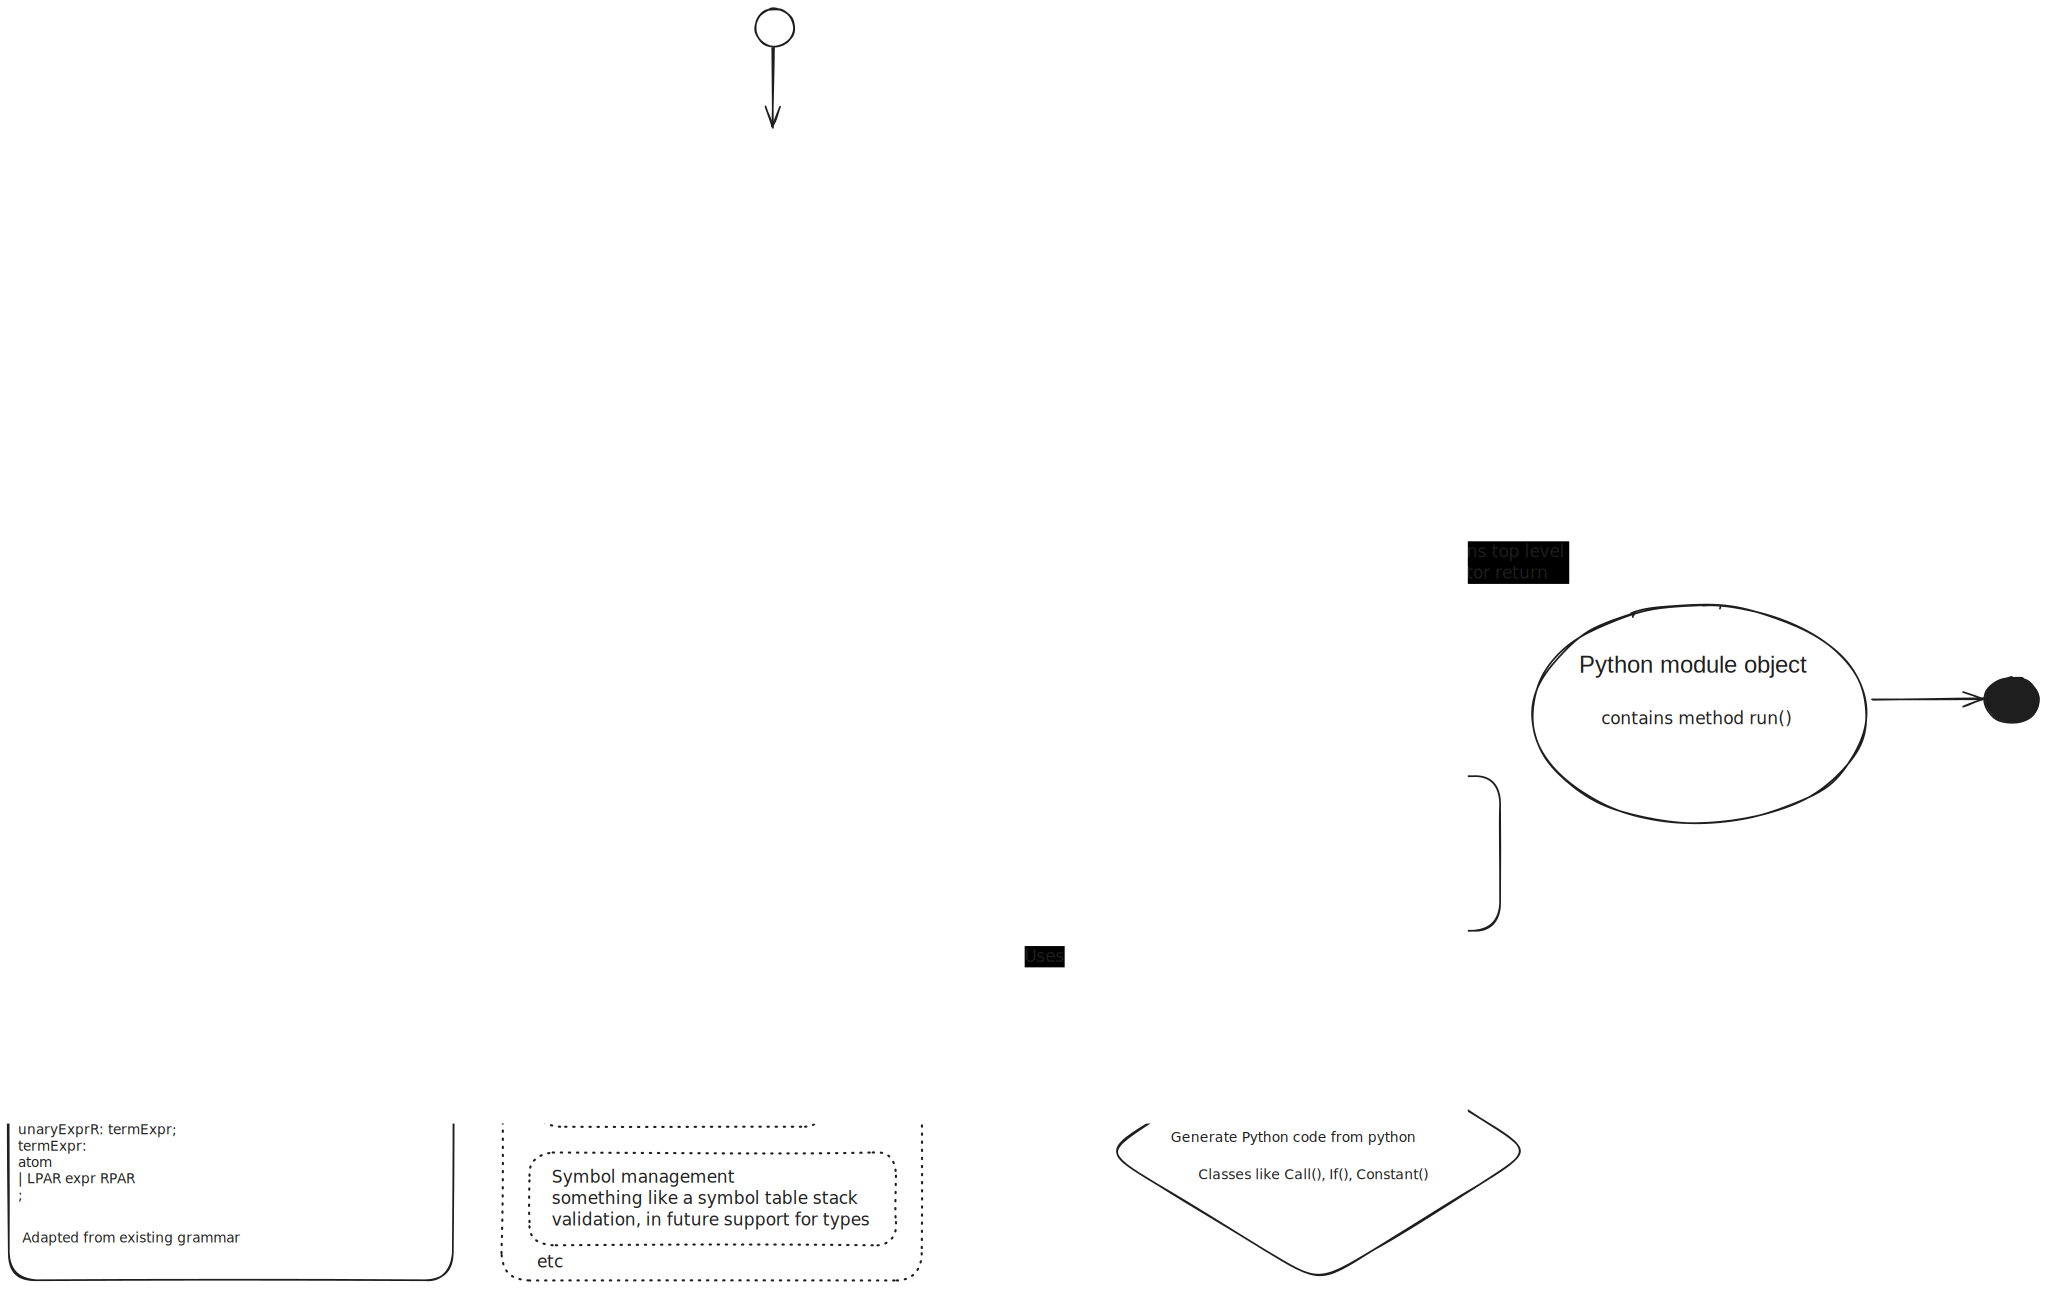
\includegraphics{img/expressions.svg}

\subsubsection{Visitor Pattern}
 From the parse tree, a visitor is generated—a component that traverses the parse tree. This visitor uses the visitor design pattern to execute operations based on the nodes of the parse tree. For the expression language, the visitor's primary role is to transform the parse tree into an Abstract Syntax Tree (AST) using Python’s ast module, which can then be executed or evaluated in a Python environment.

The following code snippet provides an example of how the visitor pattern is used to handle an AddExpr node in the parse tree:

\begin{verbatim}
    
def visitAddExpr(self, ctx: ExpressionsParser.AddExprContext):
    if ctx.left:
        op = ctx.op.children[0].symbol.type
        if op == ExpressionsParser.PLUS:
            name = Operator.ADD.value
        elif op == ExpressionsParser.MINUS:
            name = Operator.SUB.value
        else:
            raise ValueError(f"Unknown operator: {op}")
        identifier = self.get_symbol_table().get_identifier_for_name(name, "internal", "load")
        args = [self.visit(ctx.left), self.visit(ctx.right)]
        node = self.create_call_node(identifier, ctx.start.line, ctx.stop.line, args)
        return ExpressionArgument(node)

    return self.visitChildren(ctx)

\end{verbatim}

\subsubsection{Error Handling}

Syntax errors in the expressions are handled using ANTLR's error listeners. These listeners are customized to provide meaningful error messages that help in identifying and correcting syntax issues in the input expressions.

\subsection{Statements}

Handling variables and functions within expressions involves maintaining a symbol table where each variable's name and value are stored. Variables are parsed and evaluated through the visitor, which checks the symbol table to resolve their values during the execution of expressions.

 The symbol table keeps track of all symbols used in expressions. It ensures that each variable is correctly declared and used within its scope. Additionally, symbol transformation is employed to prevent collisions and ensure that variable names are unique within the global execution context.

 \subsection{Functions and Operators}

Implementing functions and operators in the Python version of the Ataccama Expression Language involves defining Python functions that correspond to each function and operator in the original language.

Each function from Ataccama’s language is mapped to a Python function. These functions handle various data types and perform the necessary computations or data manipulations as defined in the Ataccama language specifications.

Each operator is mapped to a function call with the operand(s) as the arguments. This allows for customizing behavior for arithmetic, logical, and comparison operations to closely align with how they function in the original implementation.

The reimplementation of the functions and operators constitutes a significant portion of the work, as the language supports a wide range of operations that need to be accurately translated to Python.

\subsection{Additional Features and Utilities}

In addition to the core features of the Ataccama Expression Language, several utilities and enhancements are implemented.

\subsubsection{Command Line Interface (CLI)}

A command-line interface is developed to allow users to interact with the expression evaluation engine directly. This CLI provides a simple way to input expressions and receive the output, making it easier to test and validate the implementation.

Running `poetry install` will make the `evaluate-records` script available.
`evaluate-records` can be used to evaluate records on a expression:

\begin{verbatim}
echo "John,25\nJohn,18" | evaluate-records "name == 'John' and
 age > 20" --record-format "name:STRING,age:INTEGER"
\end{verbatim}

\subsubsection{Expression Generator}

An expression generator is created to produce random expressions based on the grammar of the Ataccama Expression Language. This tool is useful for testing the parser and visitor components.

\section{Testing and Validation}
% Explain how you tested the reimplementation of DQ rules to ensure they work correctly and efficiently in local Python environments.

Testing and validation are critical components of the software development process, especially when reimplementing data quality (DQ) rules to ensure they perform as expected in local Python environments. For this project, we employ pytest with test parametrization to thoroughly test the Python implementation of Ataccama DQ rules.


Use of test Parametrization allows for running the same test function with different input values. It is particularly useful in this project for applying a wide array of test scenarios to the implemented functions to ensure comprehensive coverage and that the rules behave as intended across diverse data sets and conditions.

The primary focus during testing is to ensure that the reimplemented rules behave as similarly as possible to the Ataccama Expression Language. Tests are designed to validate both typical and edge-case scenarios, ensuring the rules are robust under various data conditions.

\subsection{Tool for Output Comparison}

To validate the accuracy of the reimplementation, we have developed a test suite that compares the outputs of our Python implementation against those generated by the original Ataccama ONE Expressions Java engine. This ensures that our implementation produces results consistent with the established behavior of the rules in the Ataccama environment.

This test suite can be run programatically using a script which the pytest test suite; the suite is using a fixture for running any expression that captures it and if enabled, saves it into a file. The script executes the tests and, for a subset of them, runs the same expressions in the Ataccama ONE Desktop environment. It then compares the outputs from both implementations and highlights any discrepancies.

The output can be used to identify any inconsistencies between the original and re-implemented rules, allowing for further refinement and debugging to ensure the rules are correctly implemented.

\section{Challenges and Resolutions}
% Discuss any challenges faced during the implementation and how they were resolved.

\subsection{Date formatting strings}
\paragraph{Problem}

One of the challenges encountered during the implementation was handling date formatting strings in the Ataccama Expression Language. The original language mirrors Java date formatting patterns, which are not directly compatible with Python’s datetime module. \cite{noauthor_datetimeformatter_nodate}

\paragraph{Resolution}

To address the date formatting issue, a mapping between Java and Python date formatting patterns was created. This mapping allows the Python implementation to interpret the date formatting strings correctly and convert them to the appropriate Python format.

To perform this mapping, a separate grammar with lexer and parser were added to parse the original date formatting string into pattern and text tokens. Pattern tokens are then converted using a lookup table.

\subsection{Multiline lambda functions}

\paragraph{Problem}

Another challenge was implementing multiline lambda functions in Python. The Ataccama Expression Language supports multiline lambda functions, which are not directly supported in Python. This required finding a workaround to enable multiline lambda functions in the Python implementation.

\paragraph{Resolution}

The solution involved defining full-fledged functions instead of using lambda expressions for multiline needs. To integrate these functions seamlessly and avoid namespace conflicts, we employed a symbol table that manages and mangles names dynamically. This approach ensures that all function names are unique and avoids identifier collisions within the Python environment, effectively replicating the flexibility of Ataccama's multiline lambdas within Python's syntactic constraints.
\subsection{Lookup Files}
\paragraph{Problem}

Ataccama's expressions can perform lookups against reference data stored in proprietary binary formats with sophisticated hashing strategies. This feature is crucial for validating data against predefined sets which are optimized for performance in Ataccama's native environment.
\paragraph{Solution}

To handle this, the proprietary lookup functionality was reimplemented in Python. This involved developing a method to read and interpret the binary format into a usable form in Python. Additionally, to mimic the fixed-size arithmetic and specialized hashing used by Ataccama, similar algorithms were implemented in Python, ensuring that the lookup performance remains efficient and consistent with the original implementation.
\subsection{Null Handling}
\paragraph{Problem}

Ataccama's functions and operators are designed to handle null values gracefully, often returning null or a neutral value when encountering nulls in expressions. This feature is essential for maintaining data integrity and ensuring robust data quality checks.
\paragraph{Solution}

The Python implementation adopted a similar approach to null handling. Custom operators and functions were developed to replicate the behavior of Ataccama's handling of nulls. For example, custom implementations of addition (+) and other operators were created to return null or appropriate neutral values when encountering null inputs. This ensures that the data quality rules continue to function predictably and effectively even when faced with incomplete or missing data.

This careful replication of functionality ensures that the Python version of Ataccama's DQ rules maintains the robustness and reliability of the original system, adhering closely to its operational logic and data handling practices.

\chapter{Viability Analysis}


\section{Introduction to Performance Testing}

\subsection{Purpose of Testing}


Performance testing is crucial in assessing the viability of the Python implementation of the Ataccama Expression Language, particularly in ensuring it can efficiently and effectively handle data quality rules within Python environments. This testing is not about matching the performance of similar solutions - Soda Core and Great Expectations -  but rather ensuring that the Python version is sufficiently efficient for practical use. The aim is to determine if the Python implementation performs within acceptable limits, where a slowdown by a factor of up to 10 times compared to the similar solutions might be considered tolerable for deployment, but a 1000 times slowdown would indicate serious efficiency issues that could render the solution impractical. By establishing these performance benchmarks, we can validate that the Python implementation meets minimum requirements for real-world applications, ensuring it is a viable alternative for data engineers who require programmatic access to Ataccama's data quality tools.

\subsection{Testing Framework}

\subsubsection{Tools and Setup}

The performance testing utilizes a structured approach where a specific data quality rule—represented in three different formats: an original Ataccama expression, a Soda Core implementation, and a Great Expectations setup—is executed across a range of dataset sizes. This method allows for a direct comparison of how well the Python implementation scales with increasing data volumes, a critical factor in many data engineering tasks.

\subsubsection{Methodology}

\paragraph{Dataset Sizes} Tests are conducted on datasets of varying sizes, starting from 10 records and scaling up to 1 or 10 million records depending on test case complexity. This range is chosen to simulate different real-world scenarios, from small, manageable datasets to large-scale data processing tasks.

\paragraph{Execution Repetition} Each test is repeated ten times to ensure consistency and reliability in the results. This repetition helps mitigate any anomalies or outliers that could affect the accuracy of the performance assessment.
The first repetition is considered a warm-up to allow the Python interpreter to optimize the code before the actual performance metrics are recorded. This approach ensures that the performance measurements are based on the optimized execution of the code - while Python is often perceived as an interpreted language that executes code directly from its high-level syntax, in practice, Python first compiles the source code into bytecode, which is a lower-level, platform-independent representation of the code. This bytecode is then executed by the Python interpreter. During the warm-up phase, the Python interpreter can perform several optimizations on this bytecode, such as type specializations, loop unrolling, conditional simplifications, and inline caching. 

\paragraph{Process Isolation} Each test run is executed in a freshly started Python process to avoid any potential interference from memory leaks, memory layout, residual data, or other artifacts from previous executions. This approach ensures that each test is conducted in a clean state, providing accurate and unbiased performance measurements.

\paragraph{Measurement Metrics} The key performance metric collected during the tests is execution time. This metric provides a direct measure of how long it takes for the Python implementation to process the data quality rule on datasets of different sizes, which is essential for assessing the viability and scalability of the Python implementation.


\section{Test Environment Setup}

%     % Hardware Specifications: Describe the computer systems on which the tests are conducted, including processor speeds, memory, and network configurations if relevant.
%     % Software Configuration: Detail the versions of Python, Java, and other relevant software tools or libraries used during the tests.

This section details the hardware and software specifications of the test environment to ensure that the performance results are reproducible and relevant to typical data engineering scenarios.

\subsection{Hardware Specifications}

    The performance tests were conducted on a M1 MacBook Pro with the following specifications:

    \begin{itemize}
        \item Processor: Apple M1 10-core CPU
        \item Memory: 32 GB
        \item Operating System: macOS Sonoma 14.4.1
    \end{itemize}

    \subsection{Software Configuration}

    \paragraph{Python Version} Python 3.10 is used for all Python-related tests.
    
    \paragraph{Testing Frameworks} For execution time measurements, the \texttt{timeit} module is used.
    \paragraph{Performance Monitoring Tools} Standard module \texttt{timeit} for measuring execution timewas employed.
    \paragraph{Other Software} Relevant libraries and dependencies for each test scenario are documented and version-controlled to ensure consistency. 
    

\section{Test Cases}

%     % Selection Rationale: Explain why specific test cases were chosen to reflect real-world usage scenarios that data engineers might encounter.
%     % Test Case Descriptions: Briefly introduce each test case before a detailed analysis.

\paragraph{Test Cases Descriptions and Rationale}

The choice of test cases for evaluating the performance and viability of the reimplemented Ataccama Expression Language in Python is designed to reflect a range of real-world scenarios that data engineers commonly encounter. These test cases are selected to cover a spectrum of complexity, from relatively simple checks to more involved, multi-condition validations that interact with external data sources and complex logic. This selection ensures that the testing not only assesses basic functionality but also gauges the performance under more demanding processing conditions.

All of the test cases include listing out the failed records, which is a common requirement in \glsxtrshort{dqm} tasks. This feature is essential for identifying and addressing data quality issues efficiently, making it a key aspect of the performance evaluation.

\subsection{Test Case 1: Simple Continent Validation}

\paragraph{Description} This test involves evaluating a relatively straightforward expression that checks if the value of a 'continent' field does not belong to a predefined list of continent names. 

\paragraph{Relevance} This test case is chosen for its simplicity and its commonality in data validation tasks. It represents typical scenarios where fields within datasets are validated against a fixed set of allowable values. Testing this case helps verify the Python implementation’s ability to handle basic inclusion checks efficiently, a frequent requirement in data cleaning and standardization processes.

\subsubsection{Expressions Implementation}

\begin{verbatim}
    ( NOT ( lower(continent) in { "asia", "africa", "europe", 
    "north america", "south america", "oceania", "antarctica" } ) )
\end{verbatim}

\subsubsection{Great Expectations Implementation}

\begin{verbatim}
{
  "data_asset_type": "Dataset",
  "expectation_suite_name": "default",
  "expectations": [
    {
      "expectation_type": "expect_column_values_to_be_in_set",
      "kwargs": {
        "column": "continent_lower",
        "mostly": 1,
        "value_set": [
          "asia",
          "africa",
          "europe",
          "north america",
          "south america",
          "oceania",
          "antarctica"
        ]
      },
      "meta": {}
    }
  ],
  "ge_cloud_id": null,
  "meta": {
    "great_expectations_version": "0.18.12"
  }
}
\end{verbatim}

\subsubsection{Soda Core Implementation}

\begin{verbatim}
checks for continents:
    - invalid_count(continent_lower) = 0:
          valid values: ["asia", "africa", "europe", "north america", 
                         "south america", "oceania", "antarctica"]
\end{verbatim}


\subsection{Test Case 2: Complex Customer Validation}

\paragraph{Description} This more complex test case applies multiple conditions to validate customer data, involving null checks, file lookups, regex pattern matching.

\paragraph{Relevance} This test case is designed to simulate the complex validation processes often required in customer data management, where multiple fields need to be verified against various conditions. It tests the system’s capacity to execute multiple, diverse operations — from file lookups to regular expressions and string manipulations — which are typical in scenarios involving data integration and compliance checks. It provides a robust challenge to the system, testing its performance and accuracy under load and complex logic conditions.


\section{Performance Analysis}

%     Metrics Collected: List the metrics that will be evaluated, such as execution time, memory usage, and CPU utilization.
%     Comparative Analysis: Present a detailed comparison of the performance metrics obtained from the Python implementation against those from the original Java version.

\xxx{TODO}

\section{Discussion}

%     Interpretation of Results: Discuss the implications of the test results for the viability of the Python implementation in real-world applications.
%     Potential Bottlenecks and Limitations: Identify any performance bottlenecks or limitations observed during testing and suggest possible explanations or solutions.

\xxx{TODO}


\chapter*{Conclusion}
\addcontentsline{toc}{chapter}{Conclusion}

\xxx{The conclusion should summarize the main findings of the thesis and provide a reflection on the work done. It should also discuss the implications of the results and suggest possible directions for future research.}


%%% Bibliography
\include{bibliography}

%%% Figures used in the thesis (consider if this is needed)
\listoffigures

%%% Tables used in the thesis (consider if this is needed)
%%% In mathematical theses, it could be better to move the list of tables to the beginning of the thesis.
\listoftables

%%% Abbreviations used in the thesis, if any, including their explanation
%%% In mathematical theses, it could be better to move the list of abbreviations to the beginning of the thesis.

\printglossary[type=\acronymtype]

%%% Doctoral theses must contain a list of author's publications
\ifx\ThesisType\TypePhD
\chapwithtoc{List of Publications}
\fi

%%% Attachments to the thesis, if any. Each attachment must be referred to
%%% at least once from the text of the thesis. Attachments are numbered.
%%%
%%% The printed version should preferably contain attachments, which can be
%%% read (additional tables and charts, supplementary text, examples of
%%% program output, etc.). The electronic version is more suited for attachments
%%% which will likely be used in an electronic form rather than read (program
%%% source code, data files, interactive charts, etc.). Electronic attachments
%%% should be uploaded to SIS. Allowed file formats are specified in provision
%%% of the rector no. 72/2017. Exceptions can be approved by faculty's coordinator.
\appendix
\chapter{Attachments}


\section{List of Functions}

\begin{itemize}
    \item Bitwise functions
    \begin{itemize}
        \item bitand 
        \item bitneg 
        \item bitor 
        \item bitxor 
    \end{itemize}
    \item Coding functions
    \begin{itemize}
        \item coding.md5, encode.md5 
        \item coding.fromBase64 
        \item coding.toBase64, encode.base64 
    \end{itemize}
    \item Comparison operators
    \begin{itemize}
        \item <= 
        \item <>, != 
        \item < 
        \item =, == 
        \item > 
        \item >= 
    \end{itemize}
    \item Conditional functions
    \begin{itemize}
        
\item case 
\item decode 
\item iif 
\item nvl 
    \end{itemize}
    \item Conversion functions
    \begin{itemize}
 
\item getMilliseconds 
\item math.abs 
\item math.ceil, math.ceiling 
\item math.floor 
\item math.round 
\item toFloat 
\item toInteger 
\item math.longCeil, math.longCeiling 
\item math.longFloor 
\item toLong 
\item toDate 
\item toDateTime 
\item toString 
    \end{itemize}
    \item Date functions
    \begin{itemize}
        
    \item dateAdd 
    \item dateDiff 
    \item datePart 
    \item dateTrunc 
    \item getDate 
    \item now 
    \item today 
    \item getRequestTime 
    \end{itemize}
    \item Logical operators
    \begin{itemize}
       
\item AND 
\item NOT 
\item OR 
\item XOR 
    \end{itemize}
    \item Math functions
    \begin{itemize}
  
\item math.sqrt 
\item math.acos 
\item math.asin 
\item math.atan 
\item math.cos 
\item math.e 
\item math.exp 
\item math.log 
\item math.log10 
\item math.pi 
\item math.pow 
\item math.sin 
\item math.sqr 
\item math.tan 
    \end{itemize}
    \item MinMax functions
    \begin{itemize}

        \item max 
        \item min 
        \item safeMax 
        \item safeMin 
    \end{itemize}
    \item Set operators
    \begin{itemize}
        \item is in 
        \item in 
        \item not in 
        \item is not in 
    \end{itemize}

    \item TODO rest
\end{itemize}


 is

[is not](https://www.notion.so/is-not-048f4061225140f3bcbd4142f5b98c6e?pvs=21)

[getParameterValue](https://www.notion.so/getParameterValue-4492da25bd2d4213a9f471c722df1f17?pvs=21)

[getRuntimeVersion](https://www.notion.so/getRuntimeVersion-02d29b704b9c4654a69b67392d930d18?pvs=21)

[setParameterValue](https://www.notion.so/setParameterValue-8583c79e75b847c48c02020bb284a2c8?pvs=21)

[set.contains](https://www.notion.so/set-contains-d20b2ca78c2446c199951bf72e3bc47e?pvs=21)

[set.containsExp](https://www.notion.so/set-containsExp-c6c0cdc354524c63abb3807eb93b5783?pvs=21)

[set.distinct](https://www.notion.so/set-distinct-79817147356b41ca90942c0ce097e856?pvs=21)

[set.distinctExp](https://www.notion.so/set-distinctExp-abc3a3fcb1004bc8b0c5a89f85e7ca08?pvs=21)

[set.filterExp](https://www.notion.so/set-filterExp-13fa9e8daf524374b6bbbd0d5d575131?pvs=21)

[set.indexOf](https://www.notion.so/set-indexOf-31e0238e0f8c439ab640a3d8d8a8dc84?pvs=21)

[set.indexOfExp](https://www.notion.so/set-indexOfExp-e56d0be568e14187bc5a83f1204a424f?pvs=21)

[set.item](https://www.notion.so/set-item-4a0064b788c24644921b3c62b68eb007?pvs=21)

[set.lastIndexOf](https://www.notion.so/set-lastIndexOf-9bb61ab304e14803bc6e0028c44b9660?pvs=21)

[set.lastIndexOfExp](https://www.notion.so/set-lastIndexOfExp-580473483cfb4aa3be3d12d8a9a9459b?pvs=21)

[set.mapExp](https://www.notion.so/set-mapExp-bd5ed79b71a043c69e744b7f0c7b93ba?pvs=21)

[set.size](https://www.notion.so/set-size-b28d80d9e5ff4a638373d44f2959a77f?pvs=21)

[set.sort](https://www.notion.so/set-sort-29d0175c93fa417bb352759f36d8c20e?pvs=21)

[set.subSequence](https://www.notion.so/set-subSequence-d4e25fd7eb9a4456bd76ffcc08351800?pvs=21)

[set.sumExp](https://www.notion.so/set-sumExp-d77f3b4cbade4d93a4b5d049a75dcdab?pvs=21)

[set.approxSymmetricDifference](https://www.notion.so/set-approxSymmetricDifference-2395d8d4c9134366955b19190d0c6fe2?pvs=21)

[set.difference](https://www.notion.so/set-difference-a3a5869062c24405aa17b6ffb65cd4b1?pvs=21)

[set.differenceExp](https://www.notion.so/set-differenceExp-0362b2808e094fccacd9fc8240beb526?pvs=21)

[set.differenceResult](https://www.notion.so/set-differenceResult-2be276516e734dc2932365628d0606d0?pvs=21)

[set.differenceResultExp](https://www.notion.so/set-differenceResultExp-450236ab208f4442837398f55b17bf14?pvs=21)

[set.intersection](https://www.notion.so/set-intersection-91d1a1aa8ed0474baa37b7541d9b4c89?pvs=21)

[set.intersectionExp](https://www.notion.so/set-intersectionExp-cd202abc864d433397f58a5f8b375e66?pvs=21)

[set.intersectionResult](https://www.notion.so/set-intersectionResult-d8ad2a860e1c466d8fb5349a3e66736e?pvs=21)

[set.intersectionResultExp](https://www.notion.so/set-intersectionResultExp-49a45d3f2d8c41f7be21c393071629b4?pvs=21)

[set.lcsDifference](https://www.notion.so/set-lcsDifference-461b62beb6574a58ae717bd7c993e872?pvs=21)

[set.lcsDifferenceExp](https://www.notion.so/set-lcsDifferenceExp-eb2b6cd3670041eb93f5f0ed8a6f4d21?pvs=21)

[set.lcsDifferenceResult](https://www.notion.so/set-lcsDifferenceResult-32d2fb3fbb1143968d758755df9a1cfa?pvs=21)

[set.lcsDifferenceResultExp](https://www.notion.so/set-lcsDifferenceResultExp-e03688ef4fb84441bac15553231a6070?pvs=21)

[set.lcsIntersection](https://www.notion.so/set-lcsIntersection-ef17fbd511884bd19907e8ef263aede5?pvs=21)

[set.lcsIntersectionExp](https://www.notion.so/set-lcsIntersectionExp-19c7e1e8af934b7ba0e4381533042172?pvs=21)

[set.lcsIntersectionResult](https://www.notion.so/set-lcsIntersectionResult-bde73c7ba6a4484c86746c651efe8f9c?pvs=21)

[set.lcsIntersectionResultExp](https://www.notion.so/set-lcsIntersectionResultExp-7680ccda49e0402bb539f4b1822befc2?pvs=21)

[set.lcsSymmetricDifference](https://www.notion.so/set-lcsSymmetricDifference-04b5e4304e9a41f3b735997d035969d7?pvs=21)

[set.lcsSymmetricDifferenceExp](https://www.notion.so/set-lcsSymmetricDifferenceExp-08f2af33f8b44896b21d9ccc85a3d6c9?pvs=21)

[set.lcsSymmetricDifferenceResult](https://www.notion.so/set-lcsSymmetricDifferenceResult-70c4972881b84ec7b6fa09ba5a6a62f7?pvs=21)

[set.lcsSymmetricDifferenceResultExp](https://www.notion.so/set-lcsSymmetricDifferenceResultExp-98da1b782c6e4d8397a180601134a96b?pvs=21)

[set.symmetricDifference](https://www.notion.so/set-symmetricDifference-56a223e903d74eb09e390e51e40d5e4d?pvs=21)

[set.symmetricDifferenceExp](https://www.notion.so/set-symmetricDifferenceExp-7fdf806274264091bf606156a015059c?pvs=21)

[set.symmetricDifferenceResult](https://www.notion.so/set-symmetricDifferenceResult-a9b3dafcc32142d682fcfa3865a111db?pvs=21)

[set.symmetricDifferenceResultExp](https://www.notion.so/set-symmetricDifferenceResultExp-790821c3870a4512a77171e956d0044b?pvs=21)

[set.union](https://www.notion.so/set-union-5bef326b282b40dca8bb298b910a0803?pvs=21)

[set.unionExp](https://www.notion.so/set-unionExp-387af33d46b54af6816044bdf3366782?pvs=21)

[set.unionResult](https://www.notion.so/set-unionResult-18443c8af5e14717893ce39049ef62f3?pvs=21)

[set.unionResultExp](https://www.notion.so/set-unionResultExp-e7ebeeb414ad4734b05416ab20997ec7?pvs=21)

[in](https://www.notion.so/in-5cdd8bc05ec74be7a6c860f7d9c552e5?pvs=21)

[is in](https://www.notion.so/is-in-2e45405500024a798accd3f27959941b?pvs=21)

[is not in](https://www.notion.so/is-not-in-351ef2174ca14cb294694175c16fb932?pvs=21)

[not in](https://www.notion.so/not-in-5effe74c6c3b472e83e85313b898884f?pvs=21)

[capitalize](https://www.notion.so/capitalize-65d84c769aa54104911567e1f4fb3495?pvs=21)

[containsWord](https://www.notion.so/containsWord-86feb3e0860140c6bf40dcd3f262e989?pvs=21)

[eraseSpacesInNames](https://www.notion.so/eraseSpacesInNames-2ea921c0692b4d16877a7f11e0199b7f?pvs=21)

[find](https://www.notion.so/find-ba9d506a251d49cab1cdcfbbdb51a48d?pvs=21)

[indexOf](https://www.notion.so/indexOf-351c952aba9047a49e4f7ca5207aaa0c?pvs=21)

[isInFile](https://www.notion.so/isInFile-f0a0d1aa05a24beca18803d622c82133?pvs=21)

[isNumber](https://www.notion.so/isNumber-2535ce7e2c3f45ed8e44342ee42f03a5?pvs=21)

[lastIndexOf](https://www.notion.so/lastIndexOf-0a5e61acd85f4fa9b03efee6a648cbf7?pvs=21)

[left](https://www.notion.so/left-00a1054eac0e4a2092ba42c63f3be302?pvs=21)

[length](https://www.notion.so/length-293a9d5a35074767bbd3bbfae641c8d0?pvs=21)

[lower](https://www.notion.so/lower-81024e5b1da748fa9a7acf27d089de45?pvs=21)

[matches](https://www.notion.so/matches-c2b081f144334ff2ba3e9e65134af2d6?pvs=21)

[removeAccents](https://www.notion.so/removeAccents-171af89c6dcd4386924dbb463b9f9a09?pvs=21)

[replace](https://www.notion.so/replace-51c5f3581eb944d5b9528f9f268d281c?pvs=21)

[right](https://www.notion.so/right-802ad8d9f1df4212b00e043b6bf98d3c?pvs=21)

[substituteAll](https://www.notion.so/substituteAll-568164257f2b429ab99432d7b41c508a?pvs=21)

[substr](https://www.notion.so/substr-7f036b73b5f749269b70135c4302736f?pvs=21)

[trashNonDigits](https://www.notion.so/trashNonDigits-c72549e179244e7e9bb5da24d36c3b95?pvs=21)

[trashNonLetters](https://www.notion.so/trashNonLetters-82f9bdca3eca4d9cbbb64a7d9fd23c18?pvs=21)

[trim](https://www.notion.so/trim-43c052d87e4d4a05b8a31c4bb6578120?pvs=21)

[trimLeft](https://www.notion.so/trimLeft-aea80ba235a9485783275274a9a07f6b?pvs=21)

[trimRight](https://www.notion.so/trimRight-9210818401ba4181b34b3a95f3b8db9f?pvs=21)

[upper](https://www.notion.so/upper-0c6ba9247b494e2f9f3608763ea9f1c4?pvs=21)

[word](https://www.notion.so/word-8171b4993ef841318ed8c4c43518a64b?pvs=21)

[wordCount](https://www.notion.so/wordCount-73f6f6670f6548229fda8b73bfee3017?pvs=21)

[*capitalizeWithException*](https://www.notion.so/capitalizeWithException-7c44c8e5c70846f2b0732129f2547cfd?pvs=21)

[countNonAsciiLetters](https://www.notion.so/countNonAsciiLetters-16a6c52582494d85b411caddc1e23e18?pvs=21)

[cpConvert](https://www.notion.so/cpConvert-f8ecbfe3a5ac41daa6f7fc201b2afd0e?pvs=21)

[distinct](https://www.notion.so/distinct-f33e587ca6894cc0960279be078721ad?pvs=21)

[editDistance](https://www.notion.so/editDistance-a6f8725c7ceb43b58c9d1053d03bd4a4?pvs=21)

[levenshtein](https://www.notion.so/levenshtein-14b47eed4cb84d70a6884586db8ee4b4?pvs=21)

[sortWords](https://www.notion.so/sortWords-a67385f5012b4f5e839f6dd24ecb11aa?pvs=21)

[squeezeSpaces](https://www.notion.so/squeezeSpaces-4cef11060f10450cb43f9813cbbbeeb8?pvs=21)

[substituteMany](https://www.notion.so/substituteMany-beca1dc7bcc348b1afe91820f6ec6670?pvs=21)

[hamming](https://www.notion.so/hamming-ccee8f42d2224fa4837ec30f8a7616a6?pvs=21)

[replicate](https://www.notion.so/replicate-6c654c6e11504c3da478cd4260f70478?pvs=21)

[transliterate](https://www.notion.so/transliterate-e69d2d086b6d43468336c546147e6199?pvs=21)

[trashDiacritics](https://www.notion.so/trashDiacritics-c800ebbc2a854b9c9949e20a74c3d790?pvs=21)

[diceCoefficient](https://www.notion.so/diceCoefficient-6f192fb3e4d44af7a8ca68ec7fbc2262?pvs=21)

[doubleMetaphone](https://www.notion.so/doubleMetaphone-b5a94d54ce64491ea55b8b95ff8f03a8?pvs=21)

[metaphone](https://www.notion.so/metaphone-5e3dfe3f20824b6b967a0297b687f340?pvs=21)

[ngram](https://www.notion.so/ngram-604d8fc1832d4ac9b106a86201280cce?pvs=21)

[preserveCase](https://www.notion.so/preserveCase-8ee292158af74a9dab1bd1d483b8b826?pvs=21)

[soundex](https://www.notion.so/soundex-ead42e2b2848490a93c6da158729d741?pvs=21)

[trashConsonants](https://www.notion.so/trashConsonants-d9efc81c4e654253ad4741c899c5ba8f?pvs=21)

[trashVowels](https://www.notion.so/trashVowels-87e14033aeb9436d84d3041ed3f02545?pvs=21)

[wordCombinations](https://www.notion.so/wordCombinations-4e91765ef74840728be3c8212425383e?pvs=21)

[jaccardCoefficient](https://www.notion.so/jaccardCoefficient-400591dd8fe646f0b324e2af0c1b432e?pvs=21)

[jaroWinkler](https://www.notion.so/jaroWinkler-72fd93b900b745da98e7db88f0b1c6bc?pvs=21)
\section{Expressions transpiler code}
\label{app:transpiler}

The expression transpiler package is the main source code package. It contains the source code, tests, documentation, and additional files.

\dirtree{%
.1 .
.2 src.
.3 ataccama.
.4 expressions\DTcomment{main code package}.
.2 tests.
.3 ataccama.
.4 expressions\DTcomment{package with pytest test suite}.
.2 examples\DTcomment{jupyter notebooks with simple examples}.
.2 docs\DTcomment{markdown files with high-level docs}.
.2 pyproject.toml\DTcomment{package file}.
.2 README.md.\DTcomment{overview with installation and usage instructions}.
.2 DEVELOPMENT.md\DTcomment{contains information about how to run tests}.
.2 poetry.lock\DTcomment{lock file with dependency versions for installation}.
}
\section{Performance analysis code}
\label{app:analysis-code}

The performance analysis is for reproduction purposes provided as code. The package has following structure:

\dirtree{%
.1 /.
.2 expressions_perf_test/. % \DTcomment{source code package for performance tests}.
.3 continent/. % \DTcomment{performance test code for the continent dataset}.
.3 customers/. % \DTcomment{performance test code for the customers dataset}.
.3 common/. % \DTcomment{common performance test code}.
.3 run_single.py. % \DTcomment{script to run a single performance test run}.
.2 requirements.txt. % \DTcomment{required Python packages for the performance tests, described in README.md}.
.2 README.md. % \DTcomment{instructions on how to run the performance tests}.
.2 results.csv. % \DTcomment{output file with performance results}.
.2 run_all.sh. % \DTcomment{main script to run all performance tests and save results into results.csv}.
}

\end{document}
